\documentclass[10pt,conference,compsocconf]{IEEEtran}

\usepackage{hyperref}
\usepackage{graphicx}	% For figure environment


\begin{document}
\title{Process Book}

\author{
  Rehan Mulakhel, Noemi Romano, Raja Soufi\\
  \textit{Department of Computer Science, EPFL Lausanne, Switzerland}
}

\maketitle

\begin{abstract}
A critical part of scientific discovery is the communication of research findings to peers or the general public. Mastery of the process of scientific communication improves the visibility and impact of research. While this guide is a necessary tool for learning how to write in a manner suitable for publication at a scientific venue, it is by no means sufficient, on its own, to make its reader an accomplished writer. This guide should be a starting point for further development of writing skills.
\end{abstract}

\section{Introduction}

Over human history, thousands and thousands of meteorites fell to the Earth ground; chunk of rock and metal disagreggating in the atmosphere, hitting the ground and causing sometimes vast disasters. 

The goal of this project is to visualize this fascinating phenomenon occurred over the last centuries by means of georeferenced location of the impacts recorded by the $Meteoritical$ $society$\footnote{Meteoritical society: http://www.meteoriticalsociety.org/}. In this visualization, our principal aim is to give a general overview of the spatio-temporal evolution of this natural phenomenon, emphasizing on the user experience and the exploration of the data. This visualization targets a general public who has not strong knowledge in the field. 


\section{Data}
\label{sec:data}
The data come from the NASA’s Open Data Portal and have been downloaded from Kaggle’s platform. The data were collected by The Meteoritical Society and contain information on all of the known meteorite landings. The dataset includes the following fields:

\begin{description}
\item[\texttt{name}] \ \\
  The name of the meteorite (typically a location, often modified with a number, year, composition, etc).
\item[\texttt{id}] \ \\
  The unique identifier for the meteorite.
\item[\texttt{nametype}] \ \\
  One of: -- \texttt{valid}: a typical meteorite -- \texttt{relict}: a meteorite that has been highly degraded by weather on Earth.
\item[\texttt{recclass}] \ \\
  The class of the meteorite; one of a large number of classes based on physical, chemical, and other characteristics.
\item[\texttt{mass}] \ \\
  The mass of the meteorite, in grams.
\item[\texttt{fall}] \ \\
   Whether the meteorite was seen falling, or was discovered after its impact; one of: -- Fell: the meteorite's fall was observed -- Found: the meteorite's fall was not observed.
\item[\texttt{year}] \ \\
  The year the meteorite fell, or the year it was found (depending on the value of fell).
\item[\texttt{reclat}] \ \\
  The latitude of the meteorite's landing.
\item[\texttt{reclong}] \ \\
  The longitude of the meteorite's landing.
\item[\texttt{GeoLocation}] \ \\
  The parentheses-enclose, comma-separated tuple that combines \texttt{reclat} and \texttt{reclong}.
\end{description}

Rows containing \texttt{NaN} values or presenting a year’s value smaller than $860$ and bigger than $2016$ (suggestion of the Kaggle’s description of the data) will not be considered in our visualization project. In addition, some of the entries having coordinates values equal to $0$ ---referring to meteorites found in Antarctica of which coordinates were not given--- will not be considered.

After the cleaning, we end up with a final number of $31,705$ over $45,716$ entries.

\section{Tools}
\label{sec:tools}

The visualization is displayed in a browser for usability reasons: users do not need to download anything. This forces the application to be split into a front-end and back-end.

\subsection{Front-end}

The dynamic suggestion appearing when typing a country is done with Bootstrap which is stored in a CDN.

Jquery is used to easily switch tabs in the statistics window.

% TODO: topojson & three

\subsection{Back-end}

To do.

\section{Evolution of visualization}
\label{sec:evolution_of_visualization}
From th

\begin{figure}[tbp]
  \centering
  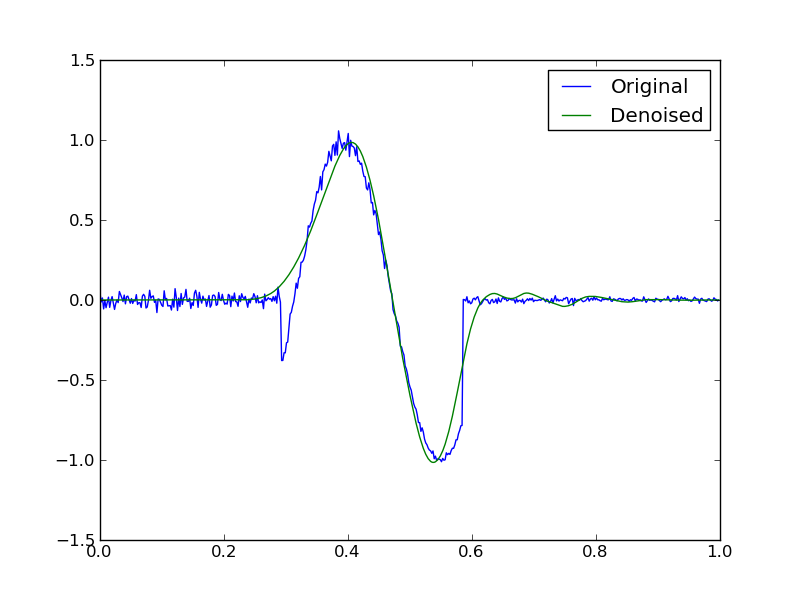
\includegraphics[width=\columnwidth]{local_wdenoised_1d}
  \vspace{-3mm}
  \caption{Signal compression and denoising using the Daubechies wavelet basis.}
  \label{fig:denoise-wavelet}
\end{figure}

Use examples and illustrations to clarify ideas and results. Figure~\ref{fig:denoise-wavelet}, we can see the two different situations where Fourier and wavelet basis perform well.

\section{Improvements}
\label{sec:improvements}

To do.

\section{Work split}
\label{sec:work_split}

\begin{description}
\item[Rehan Mulakhel] \ \\
  Web page centralizing links to the demo, code and process book. General design of the demo page. Brushing time line. Dynamic suggestion for the countries. Country to each meteorite based on coordinates.
\item[Noemi Romano] \ \\
  To do.
\item[Raja Soufi] \ \\
  To do.
\end{description}

\end{document}
